\documentclass{beamer}
%
% Choose how your presentation looks.
%
% For more themes, color themes and font themes, see:
% http://deic.uab.es/~iblanes/beamer_gallery/index_by_theme.html
%

\mode<presentation>
{
  \usetheme{default} % or try Darmstadt, Madrid, Warsaw, ...
  \usecolortheme{default} % or try albatross, beaver, crane, ...
  \usefonttheme{serif} % or try default, structurebold, ...
  \setbeamertemplate{navigation symbols}{}
  \setbeamertemplate{caption}[numbered]
}
\newcommand*\vf[1]{\mathbf{#1}}
\usepackage[english]{babel}
\usepackage[utf8x]{inputenc}
\usepackage{amsmath,mathtools,esint,bm}
\usepackage{todonotes}
\usepackage{blindtext}
\usepackage[version=3]{mhchem}
\newcommand{\mick}[1]{\textcolor{red}{[ #1 ]}}

\AtBeginSection[]{
  \begin{frame}
  \vfill
  \centering
  \begin{beamercolorbox}[sep=8pt,center,shadow=true,rounded=true]{title}
    \usebeamerfont{title}\insertsectionhead\par%
  \end{beamercolorbox}
  \vfill
  \end{frame}
}

\title[]{Charge Density Waves in Cuprates}
\author{Mick Krongchon}
\institute{University of Illinois at Urbana-Champaign}
\date{\today}

\begin{document}

\begin{frame}
\titlepage
\end{frame}

\begin{frame}{Outline}
\begin{itemize}
% \item Motivation
% \item What is a phonon?
\item Why care about charge density waves?
\item Summary of Miao and Dean's paper
\item My research
\item Conclusion
\end{itemize}
\end{frame}

\begin{frame}{Why care about charge density waves (CDWs)?}
\begin{itemize}
\item CDW is a phase transition at low $T$
\item Metals undergo a phase transition when they are cooled
\item i.e. Iron and nickel become FM. Lead and Al become superconductors
\item Since 1970s, many layered materials have been found to undergo a this type of a phase transition
\item Want to study CDW
\end{itemize}
\end{frame}

% \begin{frame}{Classical 1D chain with two masses}
% \begin{itemize}
% \item Each atom interacts only with its nearest neighbors
% \item The system equations are
% \begin{align*}
% M_1 \frac{d^2}{dt^2} u_1^l = K(u_2^l - u_1^l) - K(u_1^l - u_2^{l - 1}) = K(u_2^l - 2u_1^l + u_2^{l - 1}). \\
% M_2 \frac{d^2}{dt^2} u_2^l = K(u_1^{l + 1} - u_2^l) - K(u_2^l - u_1^l) = K(u_1^{l + 1} - 2u_2^l + u_1^l).
% \end{align*}
% \begin{figure}
% 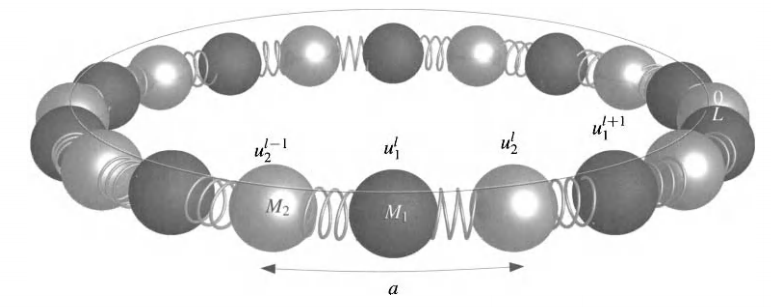
\includegraphics[width=3in]{figs/1d_diagram.png}
% \caption{\label{fig:1d_diagram}} % Alternating masses $M_1$ and $M_2$ interacting with nearest neighbors
% \end{figure}
% \end{itemize}
% \end{frame}

% \begin{frame}{Phonon branches}
% \begin{itemize}
% \item Plug in $u_j^l = A_j e^{i(kla - \omega t)}$
% \item Solve for $\omega$ that gives no trivial solutions (setting $M_2 = r M_1$):
% \begin{align}
% \omega = \sqrt{\frac{K}{M_1}}
% \sqrt{\frac{1 + r \pm \sqrt{1 + 2r\cos{ka} + r^2}}{r}}.
% \end{align}
% \begin{figure}
% 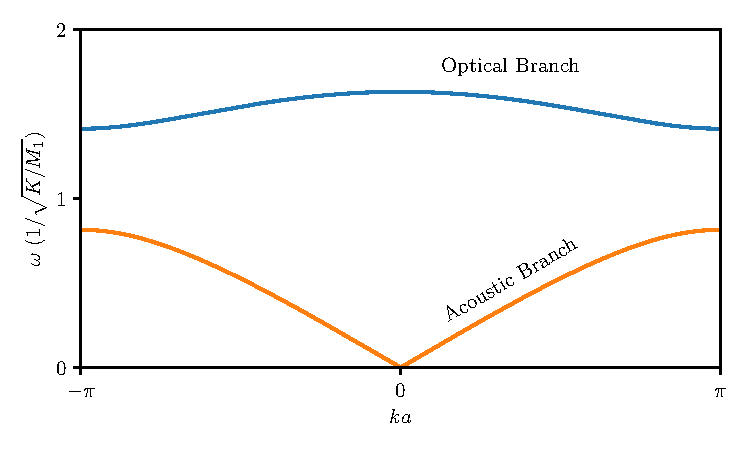
\includegraphics[width=3in]{figs/1d_dispersion.pdf}
% \caption{\label{fig:1d_dispersion} $\omega(k)$ when $r = 3$}
% \end{figure}
% \end{itemize}
% \end{frame}

% \begin{frame}{Crystalline lattices are \textbf{not} 1D chains}
% \begin{itemize}
% % \item They are not 3D mass-spring lattices either
% % \item But the idea is correct given small deviations
% % \item Let $\vf{u}^1$ ... $\vf{u}^N$ describe the displacement of ions $1$ ... $N$ from their equilibrium locations $\vf{R}^1$ ... $\vf{R}^N$
% \item Take the energy functional to be
% \begin{align*}
% \mathcal{E}(\vf{u}^1, \vf{u}^2~...~\vf{u}^N) = \mathcal{E}(u_x^1, u_y^1, u_z^1, u_x^2, u_y^2, u_z^2~...~u_x^N, u_y^N, u_z^N).
% \end{align*}
% \item The second-order Taylor series expansion around $\vf{O} = (\vf{0}^1, \vf{0}^2~...~\vf{0}^N)$ is
% \begin{align}
% \mathcal{E} &= \mathcal{E}(\vf{O}) + \sum_{\alpha,i} \frac{\partial \mathcal{E}(\vf{O})}{\partial u_\alpha^i}u_\alpha^i + \frac{1}{2} \sum_{\alpha,i} \sum_{\beta,j} \frac{\partial^2 \mathcal{E}(\vf{O})}{\partial u_\alpha^i \partial u_\beta^j} u_\alpha^i u_\beta^j, \\
% &= \mathcal{E}_c + \frac{1}{2} \sum_{\alpha,i} \sum_{\beta,j} u_\alpha^i \Phi_{\alpha \beta}^{i j} u_\beta^{j}, \label{eq:3d_energy},
% \end{align}
% where $\alpha$ and $\beta$ range over $x$, $y$, and $z$, and $i$ and $j$ range from $1$ to $N$.
% \end{itemize}
% \end{frame}

% \begin{frame}{}
% \begin{itemize}
% \item Taking the derivative to find force
% \begin{align*}
% F_x &=&&-\frac{\partial \mathcal{E}}{\partial u_x^l} = -\sum_i
% \begin{bmatrix}
% \Phi_{xx}^{li} & \Phi_{xy}^{li} & \Phi_{xz}^{li}
% \end{bmatrix}
% \begin{bmatrix}
% u_x^i & u_y^i & u_z^i
% \end{bmatrix}^\text{T}.
% \end{align*}
% \item Similarly for $F_y$ and $F_z$, the equation of motion is therefore
% \begin{align}
% \boxed{M \ddot{\vf{u}}^l = -\sum_i
% \begin{bmatrix}
% \Phi_{xx}^{li} & \Phi_{xy}^{li} & \Phi_{xz}^{li} \\
% \Phi_{yx}^{li} & \Phi_{yy}^{li} & \Phi_{yz}^{li} \\
% \Phi_{zx}^{li} & \Phi_{zy}^{li} & \Phi_{zz}^{li}
% \end{bmatrix}
% \begin{bmatrix}
% u_x^i \\
% u_y^i \\
% u_z^i
% \end{bmatrix} = -\sum_i \Phi^{li} \vf{u}^i}, \label{eq:phonon_motion}
% \end{align}
% where the subscripts are suppressed in the $3 \times 3$ matrix $\Phi^{li}$.
% \item Plug in, $\vf{u}^l = \vf{A} e^{i (\vf{k} \cdot \vf{R}^l - \omega t)}$
% \begin{align}
% M \omega^2 \vf{A} &= \sum_{l^{\prime}} \Phi^{l l^{\prime}} e^{i \vf{k} \cdot (\vf{R}^{l^{\prime}} - \vf{R}^l)} \vf{A} = \Phi(\vf{k}) \vf{A}, \label{eq:phonon_motion_matrix}
% \end{align}
% \end{itemize}
% \end{frame}

% \begin{frame}{What is charge density waves (CDW)}
% \begin{itemize}
% \item The electron density in metals is uniform
% \item The equilibrium positions form a perfectly periodic lattice
% \item When $T < T_c$, the Fermi surface becomes unstable
% \item The instability may result in periodic charge density modulation called CDW
% \item In 1950s, Fr\"{o}hlich tried to explain SC that electrons and lattices move together
% % \item No unifying description for CDW in different systems?
% \end{itemize}
% \end{frame}

\begin{frame}{Peierls' picture: 1D chain}
\begin{itemize}
% \item In 1930s, Peierls described the instability in a 1D chain of equally spaced atoms
% \item The only zero energy transition is from $k_F$ to $-k_F$, % where $k_F$ is the Fermi wave number
\item The Fermi points are at $k_F = \pm \pi / 2 a$ % connected by a vector $q = 2 k_F$
% \item The disturbance with $q = 2 k_F$ changes spacing to $2 a$
\item Gap occurs at $k = \pm \pi / 2 a$ when $T < T_c$
\item Metal-to-insulator transition at $T_c$ is called \textbf{Peierls' transition}
\begin{figure}
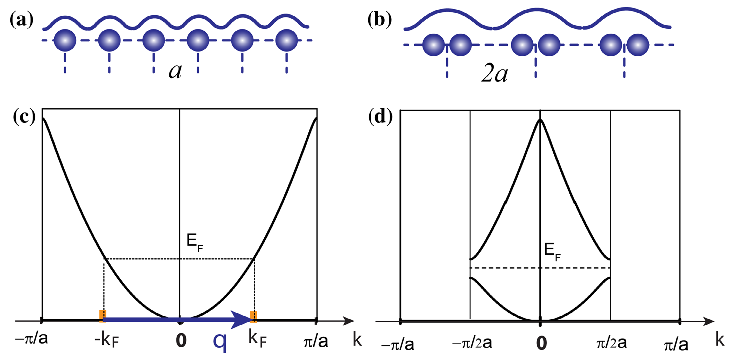
\includegraphics[width=3in]{figs/density_fermi.pdf}
\caption{\label{fig:density_fermi} (a, c) $T > T_c$ (b, d) $T < T_c$}
\end{figure}
\end{itemize}
\end{frame}

\begin{frame}{Free electron gas model}
\begin{itemize}
\item \textbf{Lindhard response function} $\chi(q)$ describes free electron gas' response
\item 1D electron gas is unstable
\begin{figure}
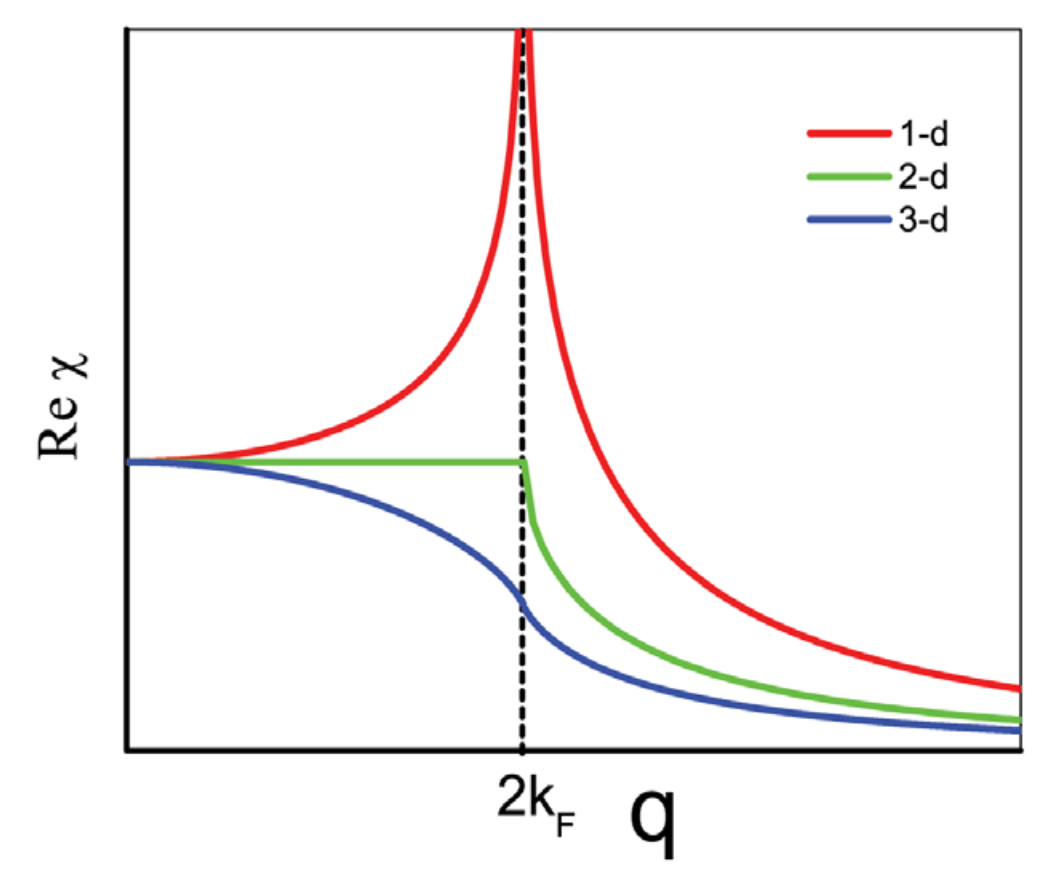
\includegraphics[width=2.5in]{figs/lindhart.png}
\caption{\label{fig:lindhart} Real part of Linhard function for 1D, 2D and 3D free electron gas models}
\end{figure}
\end{itemize}
\end{frame}

\begin{frame}{Kohn anomaly}
\begin{itemize}
\item In 1959, Kohn: The excitations at $2 k_F$ will screen any lattice motion with this wave vector
\item The phonon modes near $2 k_F$ will drop to a lower energy
\item This is called \textbf{phonon softening}
%  This strong renormalization of the phonon due to interactions with an electron system is referred to as the Kohn anomaly
\begin{figure}
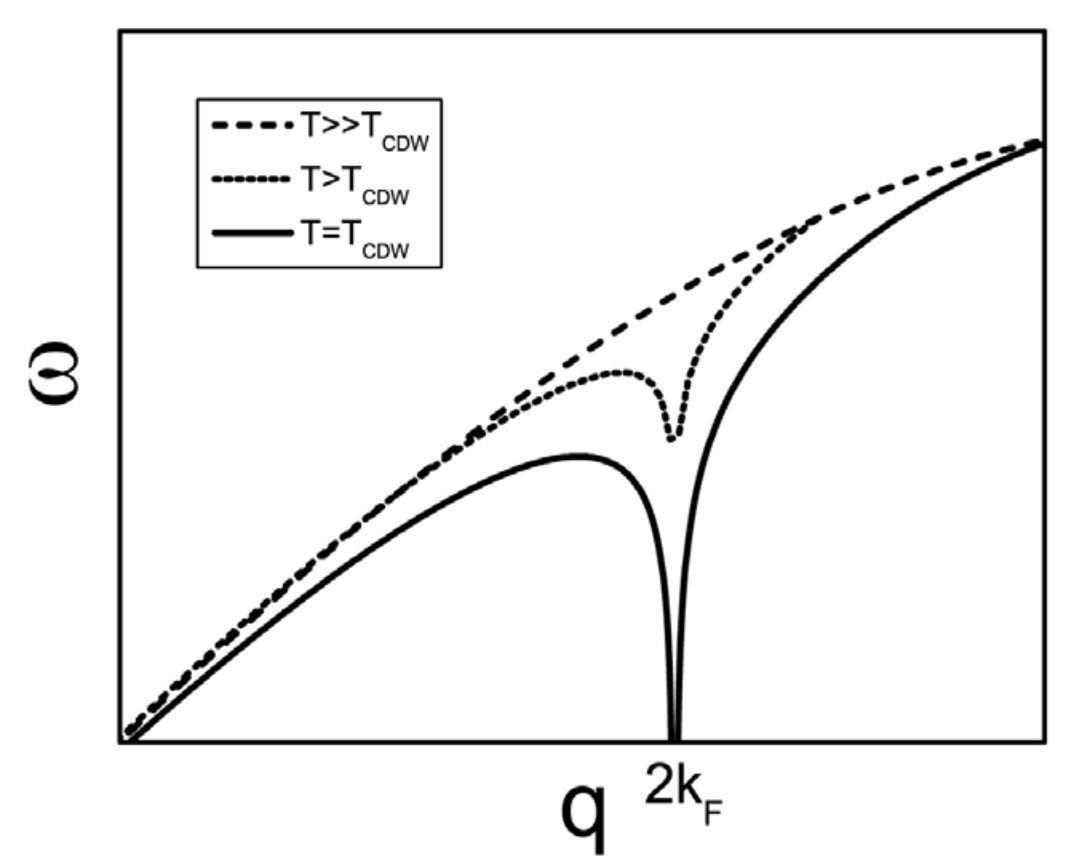
\includegraphics[width=2in]{figs/kohn_anomaly.png}
\caption{\label{fig:kohn_anomaly} Phonon energy of 1D chain at different $T$}
\end{figure}
\end{itemize}
\end{frame}

\begin{frame}{Miao and Dean's \textit{Incommensurate Phonon Anomaly and the Nature of Charge Density Waves in Cuprates} (2018)}
\begin{itemize}
\item \textit{Goal:} Find unifying description for superconducting cuprates
\item CDW instabilities are common superconducting cuprates
\item CDWs have different ordering wave vectors
\item They measured the $T$ dependence of the low-energy phonons in La$_{1.875}$Ba$_{0.125}$CuO$_4$ and compared it to YBa$_2$Cu$_3$O$_{6 + \delta}$
\end{itemize}
\end{frame}

\begin{frame}{Inelastic x-ray scattering measurement of $S(\vf{Q}, \omega)$}
\begin{itemize}
\item Why measured $S(\vf{Q}, \omega)$? ``Because they can" - Lucas
\item Dashed lines are calculated using DFPT with PBE functional
\begin{figure}
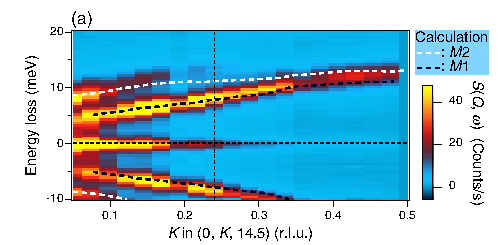
\includegraphics[width=3.5in]{figs/exp_sq.pdf}
\caption{\label{fig:exp_sq} Phonon dynamic structure factor at $T = 300~\mathrm{K}$}
\end{figure}
\end{itemize}
\end{frame}

\begin{frame}{Example fits of spectra at $K$ = 0.09, 0.23, and 0.31 r.l.u. at different $T$}
\begin{figure}
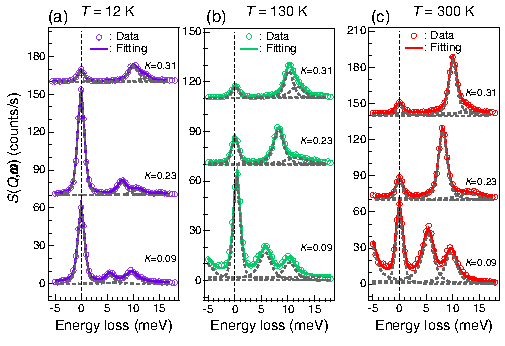
\includegraphics[width=3.5in]{figs/exp_fit.pdf}
\caption{\label{fig:exp_fit} }
\end{figure}
\end{frame}

\begin{frame}{Peaks at different $T$}
\begin{figure}
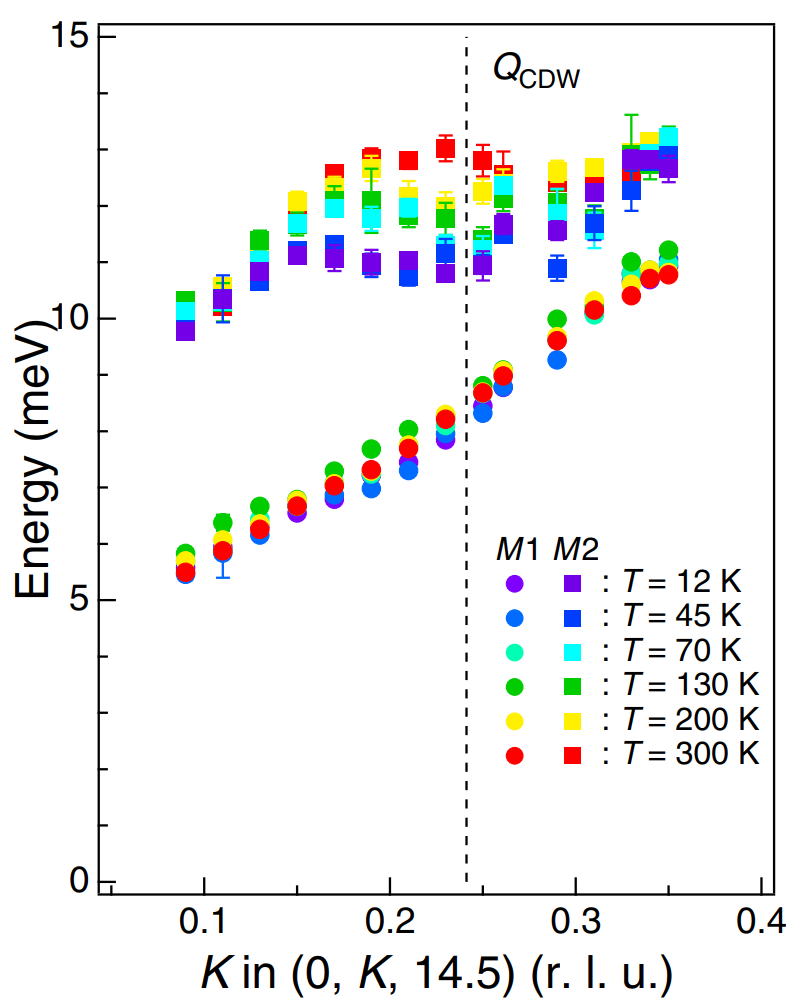
\includegraphics[width=2.2in]{figs/exp_E_k.png}
\caption{\label{fig:exp_E_k} $Q_{\text{CDW}} = 0.23~\mathrm{r.l.u.}$}
\end{figure}
\end{frame}

\begin{frame}{$T$ dependence at $K = 0.23~\mathrm{r.l.u.}$}
\begin{itemize}
\item Since they found that $M2$ has a large component of $c$-axis displacements, they suggest that $c$-axis coupled most strongly to the CDW
\begin{figure}
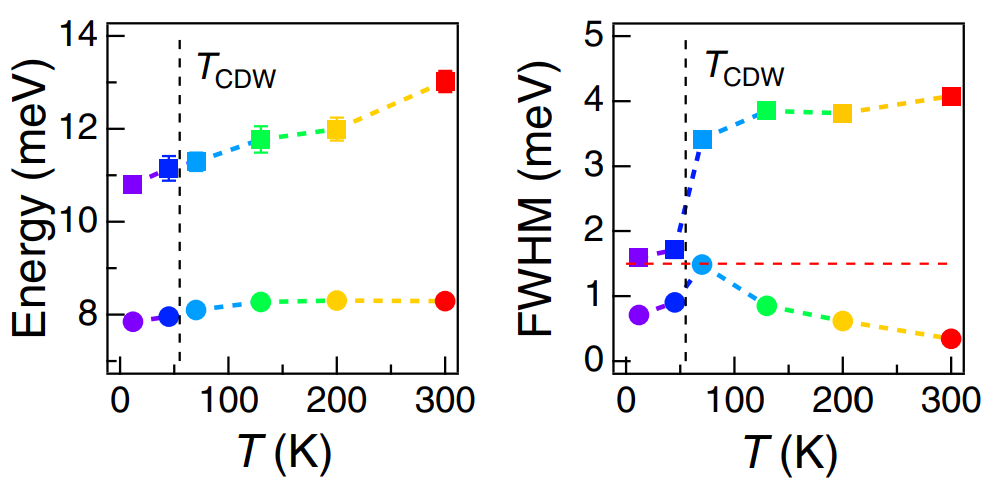
\includegraphics[width=3.5in]{figs/exp_T_dependence.png}
\caption{\label{fig:exp_T_dependence} $T_{\text{CDW}} = 55~\mathrm{K}$}
\end{figure}
\end{itemize}
\end{frame}

\begin{frame}{Maximum phonon softening moves with increasing $T$}
\begin{itemize}
\item They conclude that $Q_{\text{CDW}} = 0.238~\mathrm{r.l.u.}$ at $T = 55~\mathrm{K}$, and $Q_{\text{CDW}} = 0.3~\mathrm{r.l.u.}$ at $T = 300~\mathrm{K}$
\item Which is similar to a wave vector reported in YBa$_2$Cu$_3$O$_{6 + \delta}$
\begin{figure}
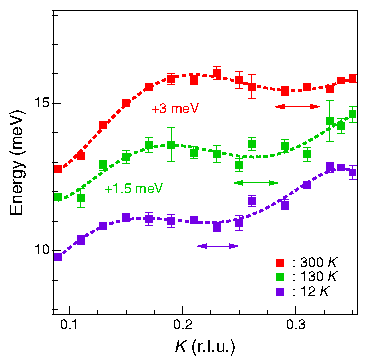
\includegraphics[width=2.5in]{figs/exp_E_k_zoomed.pdf}
\caption{\label{fig:exp_E_k_zoomed} }
\end{figure}
\end{itemize}
\end{frame}

\begin{frame}{My research}
\begin{itemize}
\item \textit{Goal:} Identify phonon-softening modes of charge density wave
\end{itemize}
\end{frame}

\end{document}
